\section{Instant Messaging}

\frame{
  \frametitle{Inhaltsverzeichnis}
  \tableofcontents[currentsection]
}

\begin{frame}
  \frametitle{Open Source vs. Closed Source}
  \begin{definition}[Open Source]
   Programm mit öffentlich zugänglichem Quellcode \hfill \tiny [Duden]
  \end{definition}

  \begin{itemize}
   \item Programm kann von jedem geprüft werden
   \item Schwer Hintertüren einzubauen
   \item Notwenige Bedingung für prüfbar sichere Programme
   \item Open Source $\neq$ kostenlos
  \end{itemize}

\end{frame}


\begin{frame}
  \frametitle{EFF Scorecard zu Messaging Apps}
  \center
  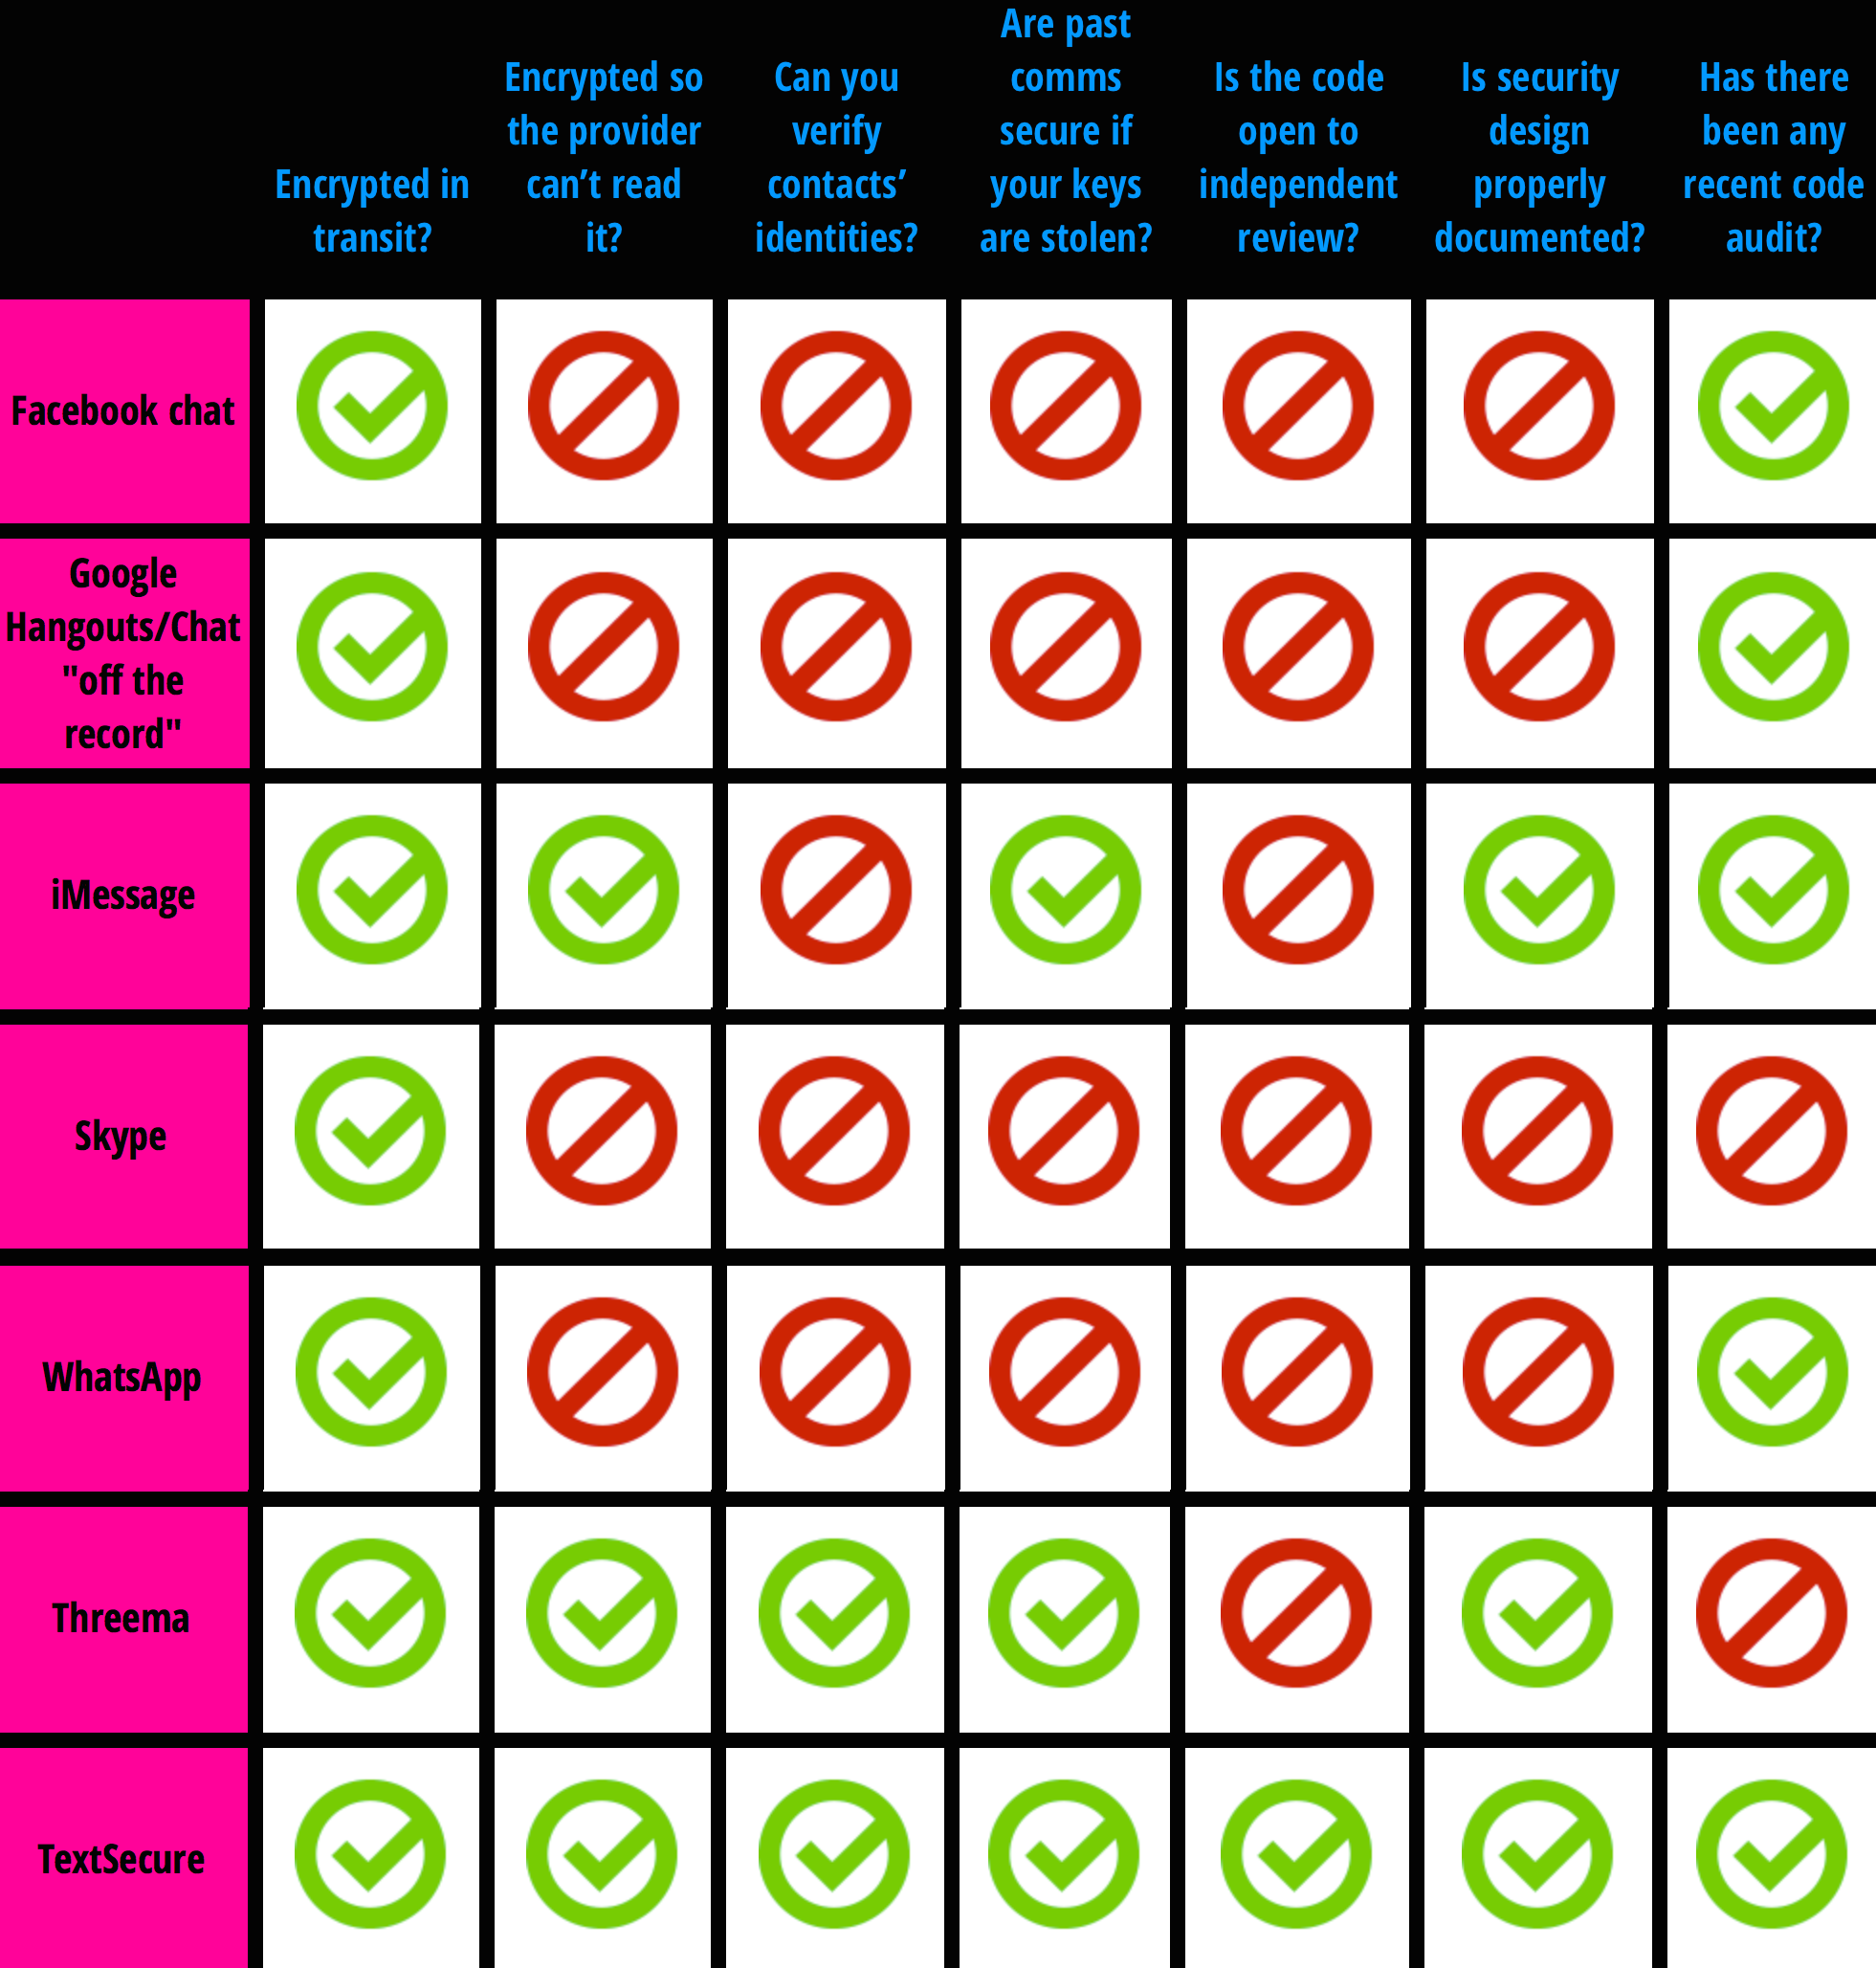
\includegraphics[width=0.6\textwidth]{figures/eff_scorecard.png}
\end{frame}

\begin{frame}
  \frametitle{Identitätsprüfung}
  \center
  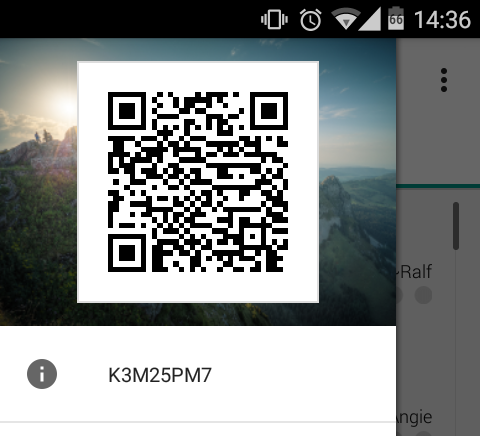
\includegraphics[width=0.6\textwidth]{figures/Threema_ID.png}
\end{frame}
